\documentclass[a4paper]{article}

\usepackage[utf8]{inputenc}
\usepackage[portuguese]{babel}	
\usepackage{graphicx}
\graphicspath{ {Imagens/} }

\title{Trabalho Prático 2 de Processamento de Linguagens}
\author{André Vieira (A78322) \and Eduardo Rocha (A77048) \and Ricardo Neves (A78764)}
\date{\today}

\begin{document}

\maketitle

\begin{abstract}
  Este documento apresenta o relatório do segundo projeto de Processamento de Linguagens, 
  de Mestrado Integrado em Engenharia Informática da Universidade do Minho.
  Aqui, será realizada a descrição de todo o trabalho realizado pelo grupo, que
  consistiu em converter um ficheiro XML para .DOT, utilizando expressões 
  regulares e Gerador FLEX.

\end{abstract}

\tableofcontents

\section{Introdução}
\label{sec:intro}

Este trabalho prático foi realizado no ambito da Unidade Curricular de Processamento de Linguagens.
Aqui, iremos dicutir toda a estratégia e linha de pensamento que o grupo tomou, de modo a cumprir os requisitos pedidos.

Uma vez que o menor número mecanográfico é igual a 77048, e ao dividir este mesmo número por 5, constatamos que o resto desta operação é igual a 3. Assim, 3+1=4, o que corresponde ao número do exercicio a realizar.

Deste modo, o grupo constatou que o enunciado atribuido foi o 2.4 - XML to Dot.
Este trabalho engloba, em geral, 2 exercícios distintos, que iremos mencionar mais à frente, em pormenor.
O objetivo máximo do grupo em relação a este trabalho foi o de realizar o exercício com a maior eficiência, ganhando, assim, experiência e conhecimento em relação às expressões regulares e o gerador FLEX, que irá ser importante no seguimento desta Unidade Curricular. 
Com o fecho da introdução deste relatório, é adequado mencionar a estrutura do mesmo. Este relatório contém o resumo do trabalho que foi realizado durante o período dado para tal, a descrição e a implementação do exercício que do trabalho prático (incluíndo a linha de pensamento seguida pelo grupo, bem como imagens que ajudam à interpretação), e no final, uma pequena conclusão que reflete o trabalho realizado.

\section{Resumo}
\label{sec:resumo}

Este trabalho prático resume-se, então, à criação e desenho de um grafo de dependencias entre elementos de um documento anotado em XML.
Para isto é necessário um ficheiro XML implementado numa estrutura semelhante à seguinte:

\begin{center}
	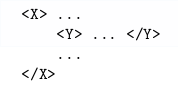
\includegraphics{enunciado1}
	\begin{figure}[!ht]
	\caption{Estrutura XML de exemplo}
	\end{figure}
\end{center}

Com um ficheiro XML dado, o grupo teria de implementar um programa que converte-se o mesmo em uma árvore documental com a estrutura de elementos. No final, a imagem do grafo respetivo seria gerada através do comando dot, no qual o grupo pesquisou acerca.
No final, o programa deverá gerar um ficheiro como este:

\begin{center}
	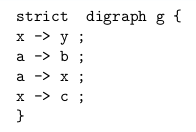
\includegraphics{enunciado2}
	\begin{figure}[!ht]
	\caption{Árvore de exemplo}
	\end{figure}
\end{center}

\section{Código FLEX}
\label{sec:flex}

Com todos os objetivos delineados, o grupo decidiu começar então a desenvolver o exercício proposto pelo professor da UC.

De seguida, iremos apresentar imagens do código desenvolvido, explicando claramente o que representam e a linha de pensamento que o grupo seguiu em cada uma delas.

O grupo, para a realização do trabalho prático, baseou-se nos exercícios realizados nas aulas práticas, nos conhecimentos adquiridos nas teóricas e em algumas pesquisas na Internet.

\begin{center}
	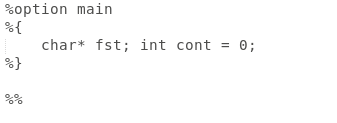
\includegraphics[scale=0.8]{flex1}
	\begin{figure}[!ht]
	\caption{Primeira imagem do exercicio desenvolvido}
	\end{figure}
\end{center}

Estas primeiras linhas de código apenas representam o início típico de qualquer programa em FLEX, com as variáveis criadas e que vão ser utilizadas mais à frente.
Aqui, o grupo criou duas variáveis, como se pode observar. O conjunto de caracteres "fst" representa o nodo principal, o nodo de cima, do ficheiro XML. O inteiro "cont" é um número que irá controlar se é necessário inserir uma seta ou um parágrafo na árvore a criar.

\begin{center}
	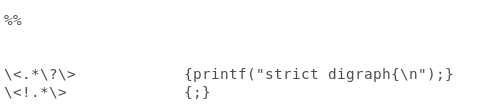
\includegraphics[scale=0.65]{flex2}
	\begin{figure}[!ht]
	\caption{Segunda imagem do exercicio desenvolvido}
	\end{figure}
\end{center}

De seguida, podemos observar duas linhas que são responsáveis por retirar as duas primeiras linhas do XML, que não são necessárias para a árvore final e, consequentemente, para o grafo do ficheiro dot.
Sendo que a primeira linha de XML termina com um ponto de interrogação e a segunda linha começa com um ponto de exclamação, torna-se relativamente fácil de apagar estas duas linhas.

\vspace{75px}
\begin{center}
	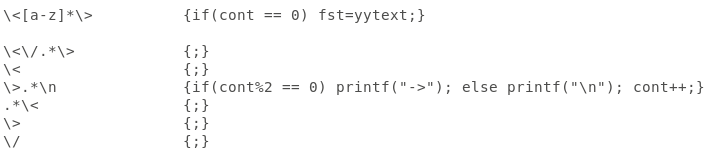
\includegraphics[scale=0.55]{flex3}
	\begin{figure}[!ht]
	\caption{Terceira imagem do exercicio desenvolvido}
	\end{figure}
\end{center}

Esta terceira parte do código pode ser considerada o verdadeiro "miolo" do código desenvolvido. Com isto, queremos afirmar que é aqui que as  linhas do código XML são realmente alteradas, de modo a transforma-lo numa árvore passível de converter em grafo.
Seguindo a ordem das linhas, iremos explicar o que cada uma faz.

A primeira linha serve para guardar o nodo principal, que engloba todos os outros nodos mais pequenos. Este texto é guardado na variavel fst, quando o cont é igual a 0, ou seja, ainda não foram encontrados outros nodos.

A segunda linha é responsável por retirar todos os nodos que se fecham, por exemplo, </onde>. No entanto, este nodo ainda aparece no ficheiro final.

A terceira linha apenas retira o simbolo "menor que" dos nodos.

A quarta linha retira o texto que não será necessário para a árvore final. Isto é, o texto que se encontra entre a abertura e o fecho de um nodo. Para além disto, se "cont" for par, coloca uma nova seta, se for impar, cria um parágrafo.

A antepenúltima linha é um complemento da função da anterior, ou seja, retira texto desnecessário.

A sexta linha retira o simbolo "maior que" dos nodos.

A ultima linha retira a barra "/", presente nos nodos de fecho.

\begin{center}
	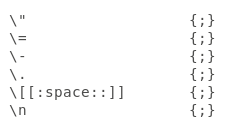
\includegraphics{flex4}
	\begin{figure}[!ht]
	\caption{Quarta imagem do exercicio desenvolvido}
	\end{figure}
\end{center}

Na quarta parte do código desenvolvido, podemos observar que serve para retirar caracteres indesejados, como as aspas, o simbolo de igual "=", o traço horizontal "-", o ponto ".", os espaços e/ou os parágrafos.

\begin{center}
	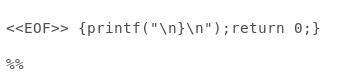
\includegraphics{flex5}
	\begin{figure}[!ht]
	\caption{Ultima imagem do exercicio desenvolvido}
	\end{figure}
\end{center}

Por fim, esta quinta e ultima linha de código é responsável por escrever no ficheiro final a chaveta "\}" para a representação da árvore.

Com isto tudo realizado, está na hora de testar o código escrito.

\section{Ficheiro Final}
\label{sec:ffinal}

Para facilitar o trabalho do grupo, criamos uma Makefile para tornar os testes mais rápidos, ganhando tempo em não ter de escrever todos os comandos necessários. Sendo assim, implementamos a seguinte makefile.

\begin{center}
	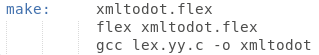
\includegraphics{makefile}
	\begin{figure}[!h]
	\caption{Makefile implementada}
	\end{figure}
\end{center}

Assim, apenas é necessário escrever o comando "make" no terminal, para proceder à compilação do ficheiro FLEX e do código C correspondente.

\begin{center}
	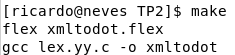
\includegraphics{makefileTerminal}
	\begin{figure}[!h]
	\caption{Código para correr a Makefile}
	\end{figure}
\end{center}

Criado o executável, é necessário executar o mesmo, dando o ficheiro XML ao qual nos iremos debruçar.

\vspace{75px}
\begin{center}
	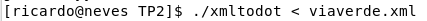
\includegraphics[scale=0.8]{xmltodotViaVerde}
	\begin{figure}[!h]
	\caption{Comando para executar o programa, com um ficheiro XML}
	\end{figure}
\end{center}

Neste relatório, iremos trabalhar com o ficheiro XML viaVerde, como forma de exemplo.

Depois de executar o comando acima, é informado no terminal a estrutura base da árvore, como podemos ver em baixo.

\begin{center}
	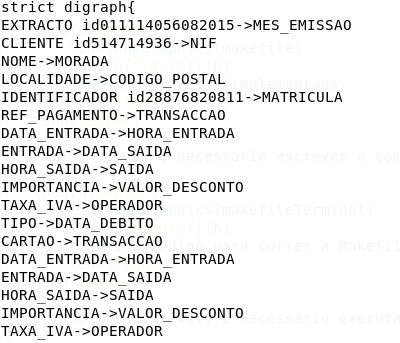
\includegraphics{arvore}
	\begin{figure}[!h]
	\caption{Excerto da estrutura da arvore}
	\end{figure}
\end{center}

Assim, basta copiar este resultado para um novo ficheiro de texto, de modo a correr um novo comando.

Depois de uma breve pesquisa na Internet, são executados os seguintes comandos.

\begin{center}
	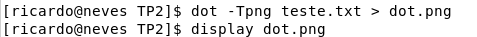
\includegraphics[scale=0.8]{comandoDot}
	\begin{figure}[!h]
	\caption{Comando para transformar um ficheiro de texto em um grafo}
	\end{figure}
\end{center}

O primeiro comando é responsável por criar uma imagem .png com o grafo correspondente à árvore resultante do ficheiro XML.
O segundo comando apenas abre uma pequena janela, de modo a visualizar a imagem desenhada anteriormente.

Assim, o resultado pode ver-se em seguida.

\begin{center}
	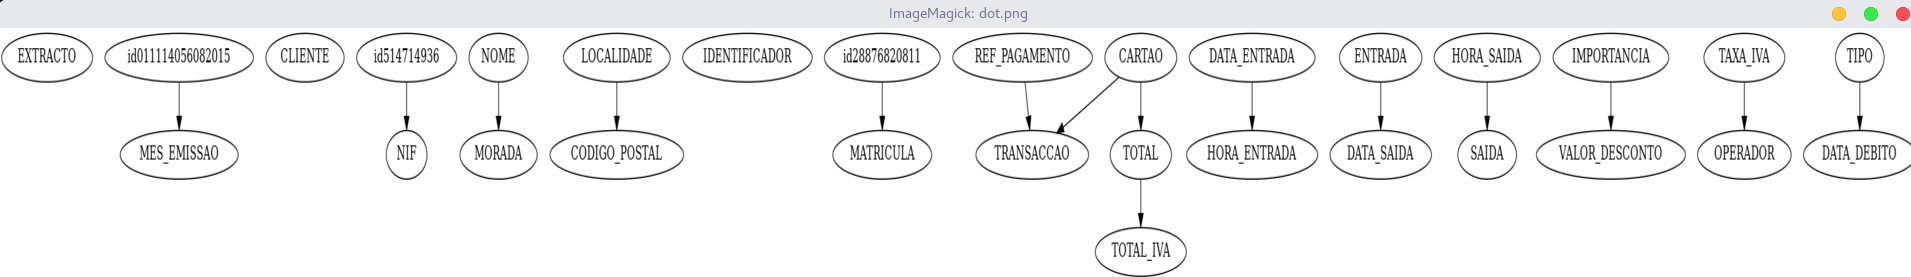
\includegraphics[scale=0.19]{dot}
	\begin{figure}[!h]
	\caption{Grafo resultante}
	\end{figure}
\end{center}

Como se pode ver acima, o resultado final não é o mais satisfatório, uma vez que o grupo sentiu uma série de dificulades na implementação do código FLEX.
As nossas dificuldades principais surgiram em repetir sempre o nodo principal, ou seja, criar a estrutura NODO PRINCIPAL -> NODO SECUNDARIO.

\section{Conclusões}
\label{sec:conclusao}

Com este trabalho prático, adquirimos e, maioritariamente, aprofundamos os nossos conhecimentos acerca do gerador FLEX. Com isto, constatamos toda a utilidade que esta ferramenta nos pode oferecer, sendo que agora, com estes exercícios, conseguimos dominar melhor a mesma.
Em suma, estamos satisfeitos com o trabalho realizado até então, sendo que o grupo se sente preparado para, após este desenvolvimento dos conhecimentos em FLEX que irão ser importantes no futuro.

\end{document}